\documentclass[submission,copyright,creativecommons]{eptcs}
\providecommand{\event}{V SUCU} % Name of the event you are submitting to
\usepackage{breakurl}             % Not needed if you use pdflatex only.
\usepackage[brazil]{babel}
\usepackage[utf8]{inputenc}  
\usepackage[T1]{fontenc}
\usepackage{graphicx,xcolor}

\title{Complexidade de Espaço}
\author{Marlon Henry Schweigert
\institute{Centro de Ciências Tecnológicas\\
Universidade do Estado de Santa Catarina\\
Joinville, Brasil}
\email{marlon.henry@edu.udesc.br}
\and
Alexandre Mendonça Fava
\institute{Centro de Ciências Tecnológicas\\
Universidade do Estado de Santa Catarina\\
Joinville, Brasil}
\email{alexandre.fava@edu.udesc.br}
}
\def\titlerunning{Complexidade de Espaço}
\def\authorrunning{Marlon Henry Schweigert \& Alexandre Fava Mendonça}
\begin{document}
\maketitle

\begin{abstract}
  Este artigo aborda o tema de complexidade de espaço, trazendo informações sobre o que é, como é medido, as classes de espaço e e complexidade de espaço existentes e as relações entre as classes existentes.
\end{abstract}

\section{Conceitos}

Complexidade de Espaço é um dos problemas recorrentes na resolução de problemas computacionais, junto a Complexidade de Tempo. A compreensão dos conceitos básicos ajudará nos tópicos futuros abordados.

\subsection{Complexidade de Espaço}

Complexidade de espaço de uma máquina de turing está relacionado a entregar uma função f a qual diga quantas células será necessário para computar algum problema.

Se a complexidade da máquina M com entrada w, sendo M uma máquina de turing decisora, podemos afirmar que o tamanho máximo utilizável da fita será f(n) para computar w.

Caso a máquina M seja uma máquina não determinista, definimos f(n) retornará o número máximo de células de todas os ramos. Ou seja, o pior caminho de computação.

\subsection{Exemplo de Complexidade de Espaço}
\label{sec:exemplo1}

L = \{W | W respeita (10)* ou (01)*\}.

Exemplos de entradas da linguagem L:

\begin{itemize}
    \item 101010
    \item 0101
\end{itemize}

Seja a MT ML decisora de L. A sua programação segue o seguinte algoritmo:

\begin{enumerate}
    \item Vá um passo a frente
    \item Repita até encontrar \_:
          \begin{enumerate}
              \item Dado o valor da cabeça na posição atual, verifique se a posição anterior possui um valor diferente.
              \item Caso seja diferente continue, caso seja igual, recuse.
              \item Avance duas casas.
          \end{enumerate}
    \item Ao encontrar \_, verifique se a ultima casa é 1. Se for 1 escreva três zeros no final e aceite.
    \item Ao encontrar \_, verifique se a ultima casa é 0. Se for 0 aceite.
\end{enumerate}

O seu pior caso pode ser considerado pela fórmula $f(n)=n+3$, visto que a entrada pertencerá a L, logo a máquina escreverá três zeros ao final.

O seu melhor caso pode ser considerado pela fórmula $g(n)=n$, visto caso a entrada não pertença a L, será recusado antes de escrever três zeros ao final.

Para as seguintes entradas temos as seguintes estimativas:

\begin{table}[!ht]
\centering
\caption{Exemplos de entrada para ML}
\label{my-label}
\begin{tabular}{|l|l|l|l|}
\hline
w & \#w & f(n) & Espaços utilizados por ML \\ \hline
1010   & 4 & 7  & 4 \\ \hline
0101   & 4 & 7  & 7 \\ \hline
101010 & 6 & 9  & 6 \\ \hline
\end{tabular}
\end{table}

\subsection{Notação de Complexidade de Espaço}

Assim como na complexidade de tempo, usaremos as principais notações. As principais são\cite{usp} $O(f(n))$ (\textit{big o}), $\Theta(f(n))$, $\Omega(f(n))$.

\colorbox{pink}{TODO}
\colorbox{yellow}{Usar definição\cite{usp}}

De forma simplista, podemos dizer que as notações de complexidade de espaço podem ser interpretadas da seguinte forma:

\begin{itemize}
    \item $O(f(n))$ refere-se ao pior caso.
    \item $\Theta(f(n))$ refere-se ao caso médio, ou onde o pior e melhor caso são iguais.
    \item $\Omega(f(n))$ refere-se ao melhor caso.
\end{itemize}

\subsection{Exemplos de notação de complexidade de espaço}

Utilizando o exemplo da máquina ML definido na seção \ref{sec:exemplo1}, temos o melhor caso definido $g(n)=n$ e o pior caso definido por $f(n)=n+3$.

Nesse exemplo, $n+3 = O(n)$ e $n = \Omega(n)$, logo o melhor e pior caso são iguais. Por esse motivo, a complexidade dessa máquina de turing será $\Theta(n)$, pois $O(n)=\Omega(n)$.

Nem sempre é fácil definir a função da complexidade média. Nesse caso conseguimos decidir facilmente pois a complexidade do pior caso e do melhor caso torna-se iguais. Porém em outros casos, podemos ter complexidades diferentes. Em casos onde o melhor e pior caso são diferentes, devemos ter a função que estima a média de todos os casos. Torna-se difícil decidir a complexidade média caso as possibilidades de entrada sejam extensas, ou até mesmo infinitas\cite{udesc}.

\section{Medição}

A forma como a complexidade de espaço é medida!

\section{Classes da complexidade de espaço}

Estimamos a complexidade de espaço por duas categorias\cite{ufpr}:

\begin{itemize}
    \item A classe P é o conjunto de todas as linguagens
decidíveis deterministicamente em tempo polinomial.
    \item A classe NP é o conjunto de todas as linguagens 
decidíveis não deterministicamente em tempo polinomial.
    \item A classe P-SPACE é o conjunto de todas as linguagens 
decidíveis deterministicamente em espaço polinomial.
    \item A classe NP-SPACE é o conjunto de todas as linguagens
decidíveis não deterministicamente em espaço polinomial.
\end{itemize}

\colorbox{pink}{TODO}
\colorbox{yellow}{Ver mais em \cite{ufpr}}

\begin{table}[!ht]
\centering
\caption{Classes de Complexidade de Espaço}
\label{my-label}
\begin{tabular}{|l|l|l|}
\hline
Classe de Complexidade & Modelo de Computação & Limitação de Recursos \\ \hline
DSPACE(f(n)) & Máquina de Turing Determinística     & Espaço f(n)     \\ \hline
L            & Máquina de Turing Determinística     & Espaço O(log n) \\ \hline
PSPACE       & Máquina de Turing Determinística     & Espaço poly(n)  \\ \hline
EXPSPACE     & Máquina de Turing Determinística     & Espaço 2poly(n) \\ \hline
NSPACE(f(n)) & Máquina de Turing Não-Determinística & Espaço f(n)     \\ \hline
NL           & Máquina de Turing Não-Determinística & Espaço O(log n) \\ \hline
NPSPACE      & Máquina de Turing Não-Determinística & Espaço poly(n)  \\ \hline
NEXPSPACE    & Máquina de Turing Não-Determinística & Espaço 2poly(n) \\ \hline
\end{tabular}
\end{table}

\begin{figure}[h]
\caption{Diagrama das classes de complexidade de espaço\cite{wiki}.}
\centering
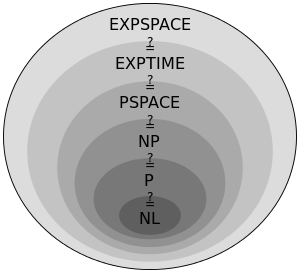
\includegraphics[width=0.5\textwidth]{pictures/classes.png}
\end{figure}

\colorbox{pink}{TODO}
\colorbox{yellow}{Adicionar mais informações de \cite{wiki}}

Existem outras classes que são definidas utilizando outras alterações de máquina de turing, como as seguintes:

\begin{itemize}
    \item BPP, ZPP e RP em máquinas de turing probabilisticas.
    \item AC e NC em circuítos booleanos.
    \item BQP e QMA em máquinas de turing quânticas.
\end{itemize}

Existem outras classes que são formadas conforme as características do problema. São alguns exemplos\cite{wiki}:

\begin{itemize}
    \item $\#P$ que é uma classe importante que inclui problemas de contagem, a qual não é um problema de decisão.
    \item $IP$ e $AM$ são classes de prova iterativa. 
    \item $ALL$ é a classe de todos os problemas de decisão.
\end{itemize}


\section{Relação entre as classes de espaço}

Loren opsum

\colorbox{pink}{TODO}
\colorbox{yellow}{Continuar lendo que P-SPACE=NP-SPACE, porém não se sabe se P=NP\cite{ufpr2}.}

\colorbox{pink}{TODO}
\colorbox{yellow}{paginas 330 do livro do Sipser\cite{sipser}.}


\section{Conclusão}

Por fim. 

\nocite{*}
\bibliographystyle{eptcs}
\bibliography{generic}
\end{document}
